\documentclass[aspectratio=169]{beamer}
% Add slides directory to search path for Dartmouth theme
\makeatletter
\def\input@path{{../}}
\makeatother
\usetheme{Dartmouth}
\usepackage{graphicx}
\usepackage{tikz}
\usepackage{amsmath}
\usepackage{listings}
\usepackage{xcolor}
\usepackage{booktabs}
% Code listing setup
\lstset{
  basicstyle=\ttfamily\small,
  keywordstyle=\color{blue},
  commentstyle=\color{gray},
  stringstyle=\color{red},
  showstringspaces=false,
  breaklines=true,
  frame=single,
  language=Python
}

\title{Classic Embeddings: LSA \& LDA}
\subtitle{Lecture 7: The Foundations of Distributional Semantics}
\author{PSYC 51.07: Models of Language and Communication - Week 3}
\date{Winter 2026}

\begin{document}

% ============================================================
% TITLE SLIDE
% ============================================================
\begin{frame}[shrink=10]
\titlepage
\end{frame}

% ============================================================
% OVERVIEW
% ============================================================
\begin{frame}[shrink=10]{Today's Lecture 📋}
\large
\begin{enumerate}\setlength{\itemsep}{0pt}
    \item 🧠 \textbf{The Distributional Hypothesis}
    \item 📊 \textbf{Vector Space Models}
    \item 📚 \textbf{Latent Semantic Analysis (LSA)}
    \item 🎲 \textbf{Latent Dirichlet Allocation (LDA)}
    \item 🎨 \textbf{Modern Topic Modeling: BERTopic}
    \item 🔍 \textbf{Evaluation \& Applications}
\end{enumerate}

\vspace{1em}
\textit{Goal: Understand how classic methods represent meaning through co-occurrence}
\end{frame}

% ============================================================
% FUNDAMENTAL QUESTION
% ============================================================
\begin{frame}[shrink=10]{The Fundamental Question 🤔}
\begin{center}
\LARGE
\textbf{How do we represent the meaning of words in a way that computers can understand?}
\end{center}

\pause
\vspace{1em}

\begin{columns}[T]
\begin{column}{0.48\textwidth}
\textbf{Traditional Approach:}
\begin{itemize}\setlength{\itemsep}{0pt}
    \item Dictionaries
    \item Taxonomies (WordNet)
    \item Manual feature engineering
    \item Knowledge bases
\end{itemize}

\vspace{0.5em}
\alert{Limitation:} Labor-intensive, hard to scale
\end{column}

\begin{column}{0.48\textwidth}
\textbf{Distributional Approach:}
\begin{itemize}\setlength{\itemsep}{0pt}
    \item Learn from data
    \item Context-based
    \item Scalable
    \item Unsupervised
\end{itemize}

\vspace{0.5em}
\alert{Key Idea:} Let the data tell us what words mean!
\end{column}
\end{columns}
\end{frame}

% ============================================================
% DISTRIBUTIONAL HYPOTHESIS
% ============================================================
\begin{frame}{The Distributional Hypothesis 📖}
\begin{center}
\huge
\textit{"You shall know a word by the company it keeps"}
\end{center}

\begin{center}
--- J.R. Firth (1957)
\end{center}

\pause
\vspace{1em}

\textbf{Key Idea:}
Words that appear in similar contexts tend to have similar meanings.

\vspace{1em}

\begin{exampleblock}{Example}
\begin{itemize}\setlength{\itemsep}{0pt}
    \item "The \textbf{cat} sat on the mat"
    \item "The \textbf{dog} sat on the mat"
    \item "The \textbf{kitten} sat on the mat"
\end{itemize}
$\rightarrow$ \textit{cat}, \textit{dog}, \textit{kitten} are semantically related
\end{exampleblock}

\vspace{0.5em}
\small
\textit{Reference: Firth, J.R. (1957). "A synopsis of linguistic theory 1930-1955"}
\end{frame}

% ============================================================
% VECTOR SPACE MODEL
% ============================================================
\begin{frame}[shrink=5]{From Words to Vectors 🗺️}
\textbf{Goal:} Represent each word as a point in high-dimensional space

\vspace{1em}

\begin{center}
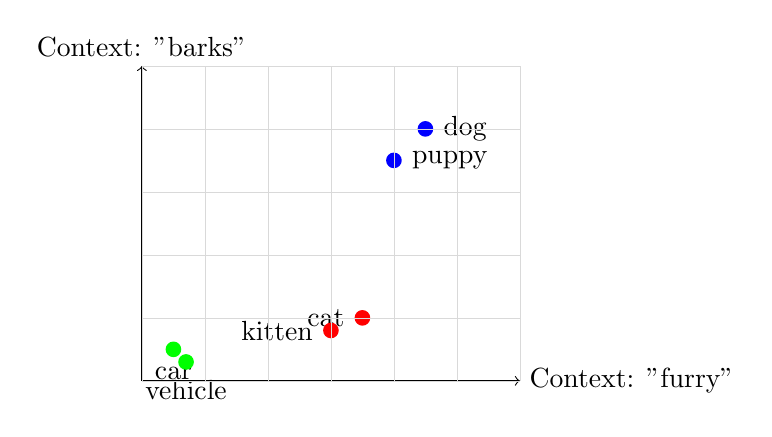
\begin{tikzpicture}[scale=0.8]
    % Axes
    \draw[->] (0,0) -- (6,0) node[right] {Context: "furry"};
    \draw[->] (0,0) -- (0,5) node[above] {Context: "barks"};

    % Points
    \node[circle,fill=blue,inner sep=2pt,label=right:{dog}] at (4.5,4) {};
    \node[circle,fill=blue,inner sep=2pt,label=right:{puppy}] at (4,3.5) {};
    \node[circle,fill=red,inner sep=2pt,label=left:{cat}] at (3.5,1) {};
    \node[circle,fill=red,inner sep=2pt,label=left:{kitten}] at (3,0.8) {};
    \node[circle,fill=green,inner sep=2pt,label=below:{car}] at (0.5,0.5) {};
    \node[circle,fill=green,inner sep=2pt,label=below:{vehicle}] at (0.7,0.3) {};

    % Grid
    \draw[help lines, gray!30] (0,0) grid (6,5);
\end{tikzpicture}
\end{center}

\textbf{Problem:} Real vocabularies have 10,000+ words, contexts are even more numerous!

$\rightarrow$ We need \textbf{dimensionality reduction} 📉
\end{frame}

% ============================================================
% TERM-DOCUMENT MATRIX
% ============================================================
\begin{frame}{Building a Term-Document Matrix 📊}
\textbf{Step 1:} Count how often each word appears in each document

\vspace{1em}

\begin{center}
\begin{tabular}{l|cccc}
\toprule
\textbf{Term} & \textbf{Doc1} & \textbf{Doc2} & \textbf{Doc3} & \textbf{Doc4} \\
\midrule
dog & 3 & 0 & 2 & 0 \\
cat & 0 & 4 & 1 & 0 \\
computer & 0 & 0 & 0 & 5 \\
code & 0 & 0 & 0 & 3 \\
animal & 2 & 3 & 2 & 0 \\
\bottomrule
\end{tabular}
\end{center}

\vspace{1em}

\textbf{Issues:}
\begin{itemize}\setlength{\itemsep}{0pt}
    \item Very sparse (mostly zeros)
    \item High dimensional (vocab size × doc count)
    \item Doesn't capture semantic relationships
\end{itemize}

\pause
\vspace{0.5em}
\alert{Solution:} Apply TF-IDF weighting and dimensionality reduction!
\end{frame}

% ============================================================
% TF-IDF
% ============================================================
\begin{frame}{TF-IDF Weighting ⚖️}
\textbf{Term Frequency - Inverse Document Frequency}

\vspace{1em}

\begin{align*}
\text{TF-IDF}(t,d) = \text{TF}(t,d) \times \text{IDF}(t)
\end{align*}

\vspace{0.5em}

\begin{columns}[T]
\begin{column}{0.48\textwidth}
\textbf{Term Frequency (TF):}
\begin{align*}
\text{TF}(t,d) = \frac{\text{count}(t,d)}{\sum_{t'} \text{count}(t',d)}
\end{align*}

How often does term $t$ appear in document $d$?

\vspace{0.5em}
\textit{Rewards frequent terms in document}
\end{column}

\begin{column}{0.48\textwidth}
\textbf{Inverse Document Frequency (IDF):}
\begin{align*}
\text{IDF}(t) = \log \frac{N}{|\{d : t \in d\}|}
\end{align*}

How rare is term $t$ across all documents?

\vspace{0.5em}
\textit{Penalizes common words like "the", "and"}
\end{column}
\end{columns}

\vspace{1em}

\begin{exampleblock}{Intuition}
Important words appear frequently in a document but rarely across all documents
\end{exampleblock}
\end{frame}

% ============================================================
% LSA
% ============================================================
\begin{frame}[shrink=10]{Latent Semantic Analysis (LSA) 📚}
\textbf{The OG of semantic embeddings (1990)}

\vspace{1em}

\begin{columns}[T]
\begin{column}{0.48\textwidth}
\textbf{Algorithm:}
\begin{enumerate}\setlength{\itemsep}{0pt}
    \item Build term-document matrix $X$
    \item Apply TF-IDF weighting
    \item Perform SVD: $X = U\Sigma V^T$
    \item Keep top $k$ dimensions
    \item Use $U_k$ as word embeddings
\end{enumerate}

\vspace{0.5em}
\textbf{Key Innovation:}
\begin{itemize}\setlength{\itemsep}{0pt}
    \item Discovers latent topics
    \item Solves synonymy problem
    \item Matrix factorization
    \item Captures semantic similarity
\end{itemize}
\end{column}

\begin{column}{0.48\textwidth}
\begin{center}
\begin{tikzpicture}[scale=0.7]
    % Term-Document Matrix
    \draw (0,0) rectangle (2,3);
    \node at (1, 3.5) {Terms};
    \node[rotate=90] at (-0.5, 1.5) {Docs};
    \node at (1, 1.5) {$X$};

    % SVD
    \node at (3, 1.5) {$=$};

    % U
    \draw (4,0) rectangle (5,3);
    \node at (4.5, 1.5) {$U$};

    % Sigma
    \draw (5.5,1.5) rectangle (7.5,3);
    \node at (6.5, 2.25) {$\Sigma$};

    % V^T
    \draw (8,1.5) rectangle (10,3);
    \node at (9, 2.25) {$V^T$};
\end{tikzpicture}
\end{center}

\vspace{0.5em}
\textbf{Matrix Interpretation:}
\begin{itemize}\setlength{\itemsep}{0pt}
    \item $U$: word-topic associations
    \item $\Sigma$: topic strengths
    \item $V^T$: topic-document associations
\end{itemize}
\end{column}
\end{columns}

\vspace{0.5em}
\small
\textit{Reference: Deerwester et al. (1990) - "Indexing by Latent Semantic Analysis"}
\end{frame}

% ============================================================
% LSA EXAMPLE
% ============================================================
\begin{frame}[shrink=10]{LSA: How It Works 🔍}
\textbf{Example: Discovering latent topics}

\vspace{1em}

\begin{columns}[T]
\begin{column}{0.48\textwidth}
\textbf{Original Dimensions:}
\begin{itemize}\setlength{\itemsep}{0pt}
    \item 50,000 terms
    \item 10,000 documents
    \item Matrix: 50k × 10k
    \item Sparse and noisy
\end{itemize}

\vspace{1em}
\textbf{After LSA:}
\begin{itemize}\setlength{\itemsep}{0pt}
    \item 100-300 latent dimensions
    \item Dense representation
    \item Captures semantic patterns
    \item Easier to compute
\end{itemize}
\end{column}

\begin{column}{0.48\textwidth}
\textbf{Discovered Topics (example):}

\vspace{0.5em}
\begin{block}{Topic 1: Technology}
computer (0.8), software (0.7), code (0.6), algorithm (0.5)
\end{block}

\begin{block}{Topic 2: Animals}
dog (0.9), cat (0.8), pet (0.7), animal (0.6)
\end{block}

\begin{block}{Topic 3: Sports}
game (0.8), team (0.7), player (0.6), win (0.5)
\end{block}

\vspace{0.5em}
\small
Words with similar topic distributions are semantically similar!
\end{column}
\end{columns}
\end{frame}

% ============================================================
% LSA LIMITATIONS
% ============================================================
\begin{frame}[shrink=10]{LSA Limitations ⚠️}
\begin{columns}[T]
\begin{column}{0.48\textwidth}
\textbf{Computational Issues:}
\begin{itemize}\setlength{\itemsep}{0pt}
    \item SVD is expensive: $O(min(nm^2, n^2m))$
    \item Hard to update with new documents
    \item Memory intensive for large corpora
\end{itemize}

\vspace{1em}
\textbf{Modeling Issues:}
\begin{itemize}\setlength{\itemsep}{0pt}
    \item Linear relationships only
    \item Bag-of-words (loses word order)
    \item No polysemy handling
    \item Negative values (hard to interpret)
\end{itemize}
\end{column}

\begin{column}{0.48\textwidth}
\textbf{Example Problem: Polysemy}

\vspace{0.5em}
\begin{exampleblock}{Word: "bank"}
\begin{enumerate}\setlength{\itemsep}{0pt}
    \item Financial institution
    \item River bank
    \item Banking (airplane maneuver)
\end{enumerate}
\end{exampleblock}

\vspace{0.5em}
LSA gives \alert{one vector} for all meanings!

\vspace{1em}
\textbf{But...}
\begin{itemize}\setlength{\itemsep}{0pt}
    \item Still useful for many tasks
    \item Foundation for modern methods
    \item Fast for medium-sized corpora
\end{itemize}
\end{column}
\end{columns}
\end{frame}

% ============================================================
% LDA INTRO
% ============================================================
\begin{frame}[shrink=10]{Latent Dirichlet Allocation (LDA) 🎲}
\textbf{A probabilistic approach to topic modeling}

\vspace{1em}

\begin{center}
\Large
\textit{What if we model documents as probabilistic mixtures of topics?}
\end{center}

\vspace{1em}

\begin{columns}[T]
\begin{column}{0.48\textwidth}
\textbf{Key Assumptions:}
\begin{enumerate}\setlength{\itemsep}{0pt}
    \item Each document is a mixture of topics
    \item Each topic is a distribution over words
    \item The mixture proportions vary per document
\end{enumerate}

\vspace{0.5em}
\textbf{Advantages over LSA:}
\begin{itemize}\setlength{\itemsep}{0pt}
    \item Probabilistic interpretation
    \item Non-negative weights
    \item Better for topic discovery
    \item More interpretable
\end{itemize}
\end{column}

\begin{column}{0.48\textwidth}
\begin{center}
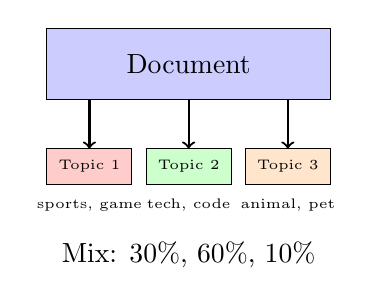
\begin{tikzpicture}[scale=0.9]
    % Document
    \draw[fill=blue!20] (0,3) rectangle (4,4);
    \node at (2, 3.5) {Document};

    % Topics
    \draw[fill=red!20] (0,1.8) rectangle (1.2,2.3);
    \node[font=\tiny] at (0.6, 2.05) {Topic 1};

    \draw[fill=green!20] (1.4,1.8) rectangle (2.6,2.3);
    \node[font=\tiny] at (2, 2.05) {Topic 2};

    \draw[fill=orange!20] (2.8,1.8) rectangle (4,2.3);
    \node[font=\tiny] at (3.4, 2.05) {Topic 3};

    % Arrows
    \draw[->, thick] (0.6, 3) -- (0.6, 2.3);
    \draw[->, thick] (2, 3) -- (2, 2.3);
    \draw[->, thick] (3.4, 3) -- (3.4, 2.3);

    % Words
    \node[font=\tiny] at (0.6, 1.5) {sports, game};
    \node[font=\tiny] at (2, 1.5) {tech, code};
    \node[font=\tiny] at (3.4, 1.5) {animal, pet};

    % Proportions
    \node at (2, 0.8) {Mix: 30\%, 60\%, 10\%};
\end{tikzpicture}
\end{center}
\end{column}
\end{columns}

\vspace{0.5em}
\small
\textit{Reference: Blei et al. (2003) - "Latent Dirichlet Allocation"}
\end{frame}

% ============================================================
% LDA GENERATIVE PROCESS
% ============================================================
\begin{frame}[shrink=10]{LDA: The Generative Story 📖}
\textbf{How LDA imagines documents are created:}

\vspace{1em}

\begin{columns}[T]
\begin{column}{0.48\textwidth}
\textbf{Generative Process:}
\begin{enumerate}\setlength{\itemsep}{0pt}
    \item Choose number of topics $K$
    \item For each topic $k$:
    \begin{itemize}\setlength{\itemsep}{0pt}
        \item Draw word distribution $\phi_k \sim \text{Dir}(\beta)$
    \end{itemize}
    \item For each document $d$:
    \begin{itemize}\setlength{\itemsep}{0pt}
        \item Draw topic distribution $\theta_d \sim \text{Dir}(\alpha)$
        \item For each word position $n$:
        \begin{itemize}\setlength{\itemsep}{0pt}
            \item Choose topic $z_{dn} \sim \text{Mult}(\theta_d)$
            \item Choose word $w_{dn} \sim \text{Mult}(\phi_{z_{dn}})$
        \end{itemize}
    \end{itemize}
\end{enumerate}
\end{column}

\begin{column}{0.48\textwidth}
\textbf{Key Parameters:}
\begin{itemize}\setlength{\itemsep}{0pt}
    \item $\alpha$: Document-topic density
    \begin{itemize}\setlength{\itemsep}{0pt}
        \item Low $\alpha$ $\rightarrow$ few topics per doc
        \item High $\alpha$ $\rightarrow$ many topics per doc
    \end{itemize}
    \item $\beta$: Topic-word density
    \begin{itemize}\setlength{\itemsep}{0pt}
        \item Low $\beta$ $\rightarrow$ focused topics
        \item High $\beta$ $\rightarrow$ general topics
    \end{itemize}
\end{itemize}

\vspace{1em}
\textbf{Inference:}
\begin{itemize}\setlength{\itemsep}{0pt}
    \item Given documents, infer topics
    \item Use Gibbs sampling or variational inference
    \item Iterative process
\end{itemize}
\end{column}
\end{columns}
\end{frame}

% ============================================================
% LDA CODE
% ============================================================
\begin{frame}[fragile]{LDA in Practice 💻}
\begin{lstlisting}[language=Python]
from sklearn.decomposition import LatentDirichletAllocation
from sklearn.feature_extraction.text import CountVectorizer

# Prepare documents
documents = [
    "The cat sat on the mat",
    "The dog ran in the park",
    "Machine learning is amazing",
    # ... more documents
]

# Create bag-of-words representation
vectorizer = CountVectorizer(max_features=1000, stop_words='english')
doc_term_matrix = vectorizer.fit_transform(documents)
vocab = vectorizer.get_feature_names_out()

# Fit LDA model
lda = LatentDirichletAllocation(
    n_components=10,  # number of topics
    random_state=42,
    max_iter=50
)

doc_topics = lda.fit_transform(doc_term_matrix)

# Print top words per topic
for idx, topic in enumerate(lda.components_):
    top_words = [vocab[i] for i in topic.argsort()[-10:]]
    print(f"Topic {idx}: {', '.join(top_words)}")
\end{lstlisting}
\end{frame}

% ============================================================
% LDA EXAMPLE
% ============================================================
\begin{frame}{LDA Example: Topic Discovery 🔍}
\begin{center}
\textbf{Example Topics from News Corpus:}
\end{center}

\vspace{1em}

\begin{block}{Topic 1: Politics (20\%)}
\texttt{government, election, president, vote, policy, senate, congress, party}
\end{block}

\begin{block}{Topic 2: Sports (15\%)}
\texttt{game, team, player, score, win, season, coach, championship}
\end{block}

\begin{block}{Topic 3: Technology (25\%)}
\texttt{software, computer, data, algorithm, system, internet, code, AI}
\end{block}

\begin{block}{Topic 4: Finance (40\%)}
\texttt{market, stock, price, investment, economy, trade, bank, profit}
\end{block}

\vspace{0.5em}
\textbf{Document representation:} [0.20, 0.15, 0.25, 0.40] $\leftarrow$ mainly finance
\end{frame}

% ============================================================
% BERTOPIC
% ============================================================
\begin{frame}[fragile]{Modern Topic Modeling: BERTopic 🎨}
\textbf{Combining neural embeddings with topic models}

\vspace{1em}

\begin{columns}[T]
\begin{column}{0.48\textwidth}
\textbf{BERTopic Pipeline:}
\begin{enumerate}\setlength{\itemsep}{0pt}
    \item Embed documents with BERT
    \item Reduce dimensionality with UMAP
    \item Cluster with HDBSCAN
    \item Generate topics via c-TF-IDF
    \item Fine-tune with MaximalMarginalRelevance
\end{enumerate}

\vspace{0.5em}
\textbf{Advantages:}
\begin{itemize}\setlength{\itemsep}{0pt}
    \item Leverages pre-trained models
    \item Better semantic understanding
    \item Automatic topic number detection
    \item Dynamic topic modeling
    \item Hierarchical topics
\end{itemize}
\end{column}

\begin{column}{0.48\textwidth}
\begin{lstlisting}[language=Python]
from bertopic import BERTopic
from sentence_transformers import SentenceTransformer

# Initialize
embedding_model = SentenceTransformer(
    "all-MiniLM-L6-v2"
)

model = BERTopic(
    embedding_model=embedding_model,
    language="english",
    calculate_probabilities=True,
    verbose=True
)

# Fit and transform
topics, probs = model.fit_transform(
    documents
)

# Get topic info
topic_info = model.get_topic_info()

# Visualize
fig = model.visualize_topics()
\end{lstlisting}
\end{column}
\end{columns}

\vspace{0.5em}
\small
\textit{Reference: Grootendorst (2022) - "BERTopic: Neural topic modeling with a class-based TF-IDF procedure"}
\end{frame}

% ============================================================
% COMPARISON
% ============================================================
\begin{frame}{LSA vs. LDA vs. BERTopic 📊}
\begin{center}
\begin{tabular}{lccc}
\toprule
\textbf{Property} & \textbf{LSA} & \textbf{LDA} & \textbf{BERTopic} \\
\midrule
Approach & Matrix factorization & Probabilistic & Neural + Clustering \\
Interpretability & Medium & High & High \\
Topic coherence & Medium & High & Very High \\
Computation & Fast & Medium & Slow \\
Scalability & Good & Good & Medium \\
Pre-training & No & No & Yes \\
Hyperparameters & Few & Many & Many \\
Topic number & Fixed & Fixed & Automatic \\
\bottomrule
\end{tabular}
\end{center}

\vspace{1em}

\begin{block}{Recommendations}
\begin{itemize}\setlength{\itemsep}{0pt}
    \item \textbf{LSA}: Quick exploration, large-scale retrieval
    \item \textbf{LDA}: Interpretable topics, when you know topic count
    \item \textbf{BERTopic}: State-of-the-art quality, exploratory analysis
\end{itemize}
\end{block}
\end{frame}

% ============================================================
% EVALUATION
% ============================================================
\begin{frame}[shrink=10]{Evaluating Topic Models 📏}
\begin{columns}[T]
\begin{column}{0.48\textwidth}
\textbf{Intrinsic Metrics:}
\begin{itemize}\setlength{\itemsep}{0pt}
    \item \textbf{Perplexity:} Lower is better
    \begin{itemize}\setlength{\itemsep}{0pt}
        \item Measures likelihood
        \item Can be misleading!
    \end{itemize}
    \item \textbf{Topic Coherence:} Higher is better
    \begin{itemize}\setlength{\itemsep}{0pt}
        \item Measures semantic similarity
        \item Better correlation with human judgment
        \item CV, UCI, UMass variants
    \end{itemize}
    \item \textbf{Topic Diversity:}
    \begin{itemize}\setlength{\itemsep}{0pt}
        \item Unique words across topics
        \item Avoids redundant topics
    \end{itemize}
\end{itemize}
\end{column}

\begin{column}{0.48\textwidth}
\textbf{Extrinsic Metrics:}
\begin{itemize}\setlength{\itemsep}{0pt}
    \item Document classification accuracy
    \item Information retrieval performance
    \item Clustering quality
\end{itemize}

\vspace{1em}
\textbf{Human Evaluation:}
\begin{itemize}\setlength{\itemsep}{0pt}
    \item Topic interpretability
    \item Word intruder detection
    \item Topic utility for task
\end{itemize}

\vspace{1em}
\begin{alertblock}{Important}
Perplexity $\neq$ usefulness!
Always check topic coherence and interpretability.
\end{alertblock}
\end{column}
\end{columns}
\end{frame}

% ============================================================
% APPLICATIONS
% ============================================================
\begin{frame}[shrink=10]{Applications of Classic Embeddings 🚀}
\begin{enumerate}\setlength{\itemsep}{0pt}
    \item \textbf{Information Retrieval}
    \begin{itemize}\setlength{\itemsep}{0pt}
        \item Semantic search
        \item Document similarity
        \item Query expansion
    \end{itemize}

    \item \textbf{Document Organization}
    \begin{itemize}\setlength{\itemsep}{0pt}
        \item Clustering
        \item Topic discovery
        \item Trend analysis
    \end{itemize}

    \item \textbf{Text Mining}
    \begin{itemize}\setlength{\itemsep}{0pt}
        \item Opinion mining
        \item Literature review
        \item Knowledge discovery
    \end{itemize}

    \item \textbf{Preprocessing}
    \begin{itemize}\setlength{\itemsep}{0pt}
        \item Feature reduction for ML
        \item Noise reduction
        \item Transfer learning
    \end{itemize}
\end{enumerate}

\vspace{0.5em}
\textbf{Real-world examples:}
\begin{itemize}\setlength{\itemsep}{0pt}
    \item Academic paper recommendations (LSA)
    \item News article categorization (LDA)
    \item Social media trend detection (BERTopic)
\end{itemize}
\end{frame}

% ============================================================
% DISCUSSION
% ============================================================
\begin{frame}[shrink=10]{Discussion Question 💬}
\begin{center}
\Large
\textbf{Can distributional semantics truly capture meaning?}
\end{center}

\vspace{1em}

\begin{columns}[T]
\begin{column}{0.48\textwidth}
\textbf{Arguments For:}
\begin{itemize}\setlength{\itemsep}{0pt}
    \item Captures semantic similarity
    \item Works well in practice
    \item Aligns with linguistic theory
    \item Scalable to large corpora
    \item Unsupervised learning
\end{itemize}
\end{column}

\begin{column}{0.48\textwidth}
\textbf{Arguments Against:}
\begin{itemize}\setlength{\itemsep}{0pt}
    \item Text-only (no grounding)
    \item Missing embodied experience
    \item No common sense reasoning
    \item Cultural context limited
    \item Reflects biases in data
\end{itemize}
\end{column}
\end{columns}

\vspace{1em}

\begin{alertblock}{The Symbol Grounding Problem}
"How can the semantic interpretation of a formal symbol system be made intrinsic to the system, rather than just parasitic on the meanings in our heads?" - Stevan Harnad (1990)
\end{alertblock}

\small
\textit{Reference: Harnad, S. (1990). "The symbol grounding problem"}
\end{frame}

% ============================================================
% PRACTICAL TIPS
% ============================================================
\begin{frame}[shrink=10]{Practical Tips 💡}
\begin{enumerate}\setlength{\itemsep}{0pt}
    \item \textbf{Preprocessing Matters:}
    \begin{itemize}\setlength{\itemsep}{0pt}
        \item Remove stopwords (but not always!)
        \item Lemmatization vs. stemming
        \item Handle punctuation carefully
        \item Consider bigrams/trigrams
    \end{itemize}

    \item \textbf{Choosing Parameters:}
    \begin{itemize}\setlength{\itemsep}{0pt}
        \item Start with 10-50 topics for LDA
        \item Use perplexity for model selection
        \item Validate with coherence scores
        \item Try multiple random seeds
    \end{itemize}

    \item \textbf{Interpreting Results:}
    \begin{itemize}\setlength{\itemsep}{0pt}
        \item Look at top 10-20 words per topic
        \item Examine representative documents
        \item Check for duplicate/junk topics
        \item Visualize with pyLDAvis
    \end{itemize}

    \item \textbf{When to Use What:}
    \begin{itemize}\setlength{\itemsep}{0pt}
        \item LSA: Fast exploration, search
        \item LDA: Interpretable topics
        \item BERTopic: Best quality, latest research
    \end{itemize}
\end{enumerate}
\end{frame}

% ============================================================
% SUMMARY
% ============================================================
\begin{frame}[shrink=10]{Summary 🎯}
\textbf{What we learned today:}

\begin{enumerate}\setlength{\itemsep}{0pt}
    \item \textbf{Distributional Hypothesis:} Words in similar contexts have similar meanings

    \item \textbf{LSA (1990):}
    \begin{itemize}\setlength{\itemsep}{0pt}
        \item SVD on term-document matrix
        \item Linear dimensionality reduction
        \item Fast but limited interpretability
    \end{itemize}

    \item \textbf{LDA (2003):}
    \begin{itemize}\setlength{\itemsep}{0pt}
        \item Probabilistic topic modeling
        \item Documents as mixtures of topics
        \item Highly interpretable
    \end{itemize}

    \item \textbf{BERTopic (2022):}
    \begin{itemize}\setlength{\itemsep}{0pt}
        \item Neural embeddings + clustering
        \item State-of-the-art coherence
        \item Automatic topic detection
    \end{itemize}

    \item \textbf{Evaluation:} Coherence $>$ perplexity

    \item \textbf{Limitation:} Static representations, no grounding
\end{enumerate}

\vspace{1em}
\begin{center}
\textbf{Next: Neural word embeddings (Word2Vec, GloVe, FastText)!}
\end{center}
\end{frame}

% ============================================================
% REFERENCES
% ============================================================
\begin{frame}[shrink=10]{Key References 📚}
\small
\textbf{Classic Papers:}
\begin{itemize}\setlength{\itemsep}{0pt}
    \item Firth, J.R. (1957). "A synopsis of linguistic theory 1930-1955"
    \item Deerwester et al. (1990). "Indexing by Latent Semantic Analysis"
    \item Blei et al. (2003). "Latent Dirichlet Allocation"
    \item Harnad, S. (1990). "The symbol grounding problem"
\end{itemize}

\vspace{0.5em}
\textbf{Modern Extensions:}
\begin{itemize}\setlength{\itemsep}{0pt}
    \item Boleda, G. (2020). "Distributional Semantics and Linguistic Theory"
    \item Grootendorst, M. (2022). "BERTopic: Neural topic modeling with a class-based TF-IDF procedure"
    \item Grand et al. (2022). "Semantic projection recovers rich human knowledge of multiple object features"
\end{itemize}

\vspace{0.5em}
\textbf{Tools \& Libraries:}
\begin{itemize}\setlength{\itemsep}{0pt}
    \item Scikit-learn: \texttt{sklearn.decomposition.TruncatedSVD}, \texttt{LatentDirichletAllocation}
    \item Gensim: \texttt{gensim.models.LsiModel}, \texttt{LdaModel}
    \item BERTopic: \texttt{https://maartengr.github.io/BERTopic/}
\end{itemize}
\end{frame}

% ============================================================
% QUESTIONS
% ============================================================
\begin{frame}{Questions? 🙋}
\begin{center}
\LARGE
\textbf{Next Lecture:}

\vspace{1em}
Word Embeddings: Word2Vec, GloVe, FastText

\vspace{1em}
\textit{From count-based to prediction-based methods!}
\end{center}
\end{frame}

\end{document}
